\documentclass[11pt,letterpaper]{article}
%\documentclass[11pt,a4paper]{report}

\usepackage{amssymb,amsmath,amsthm} 
\usepackage[margin=2cm]{geometry}
\usepackage{fancyhdr}
\usepackage{enumitem}
\usepackage[compact]{titlesec}
\usepackage{graphicx,ctable,booktabs,subfigure}

\usepackage{xparse,hyperref,parskip}

%\newcommand{\abs}[1]{\left|#1\right|}

\newcommand{\semester}{Spring 2022}
\newcommand{\due}{Tuesday, February 1}


\pagestyle{fancy}
\lhead{ }
\chead{\footnotesize Math 3338\quad  Numerical Methods\quad  \semester}
\rhead{\footnotesize \thepage}
\setlength{\parindent}{0cm}
\setlist{noitemsep}



\input{defs.tex}

%Defines the problem environment with arguments Points and Solution gap
\input{problem_env.tex}



\begin{document}

\begin{center}
{\huge{\bf  Numerical Methods}} \\[1.5ex]
{\bf Math 3338 -- \semester}\\[1.5ex]
{\Large{\bf Worksheet 5\ \\[2ex] Pointers, $\lambda$s and Weirdness}}\\
\end{center}
\vspace{2mm}

\section{Reading}

\begin{table}[!ht]
 \centering
 \begin{tabular}{ll}
   CP &  \\
 NMEP & 
 \end{tabular}
\caption{Sections Covered}
\end{table}


\section{Pointers and Weirdness}
Without using a computer, make a prediction about what the following will display,
\begin{verbatim}
L = [1,2,3]
G = L

print(G) #What does this output?

G[0] = 10

print(G) #What does this output?

print(L) #What does this output?

\end{verbatim}
Make a prediction, then test it. Try to explain why this happened.

Python uses a lot of pointers. A pointer is a reference to a location in memory. When we wrote 
$G=L$, we're really saying that $G$ and $L$ look at the same location in memory, see Figure 
\ref{fig:pointer}.
\begin{figure}[!ht]
 \centering
 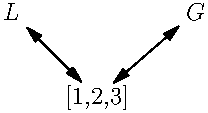
\includegraphics{images/pointer.pdf}
 \caption{Both $L$ and $G$ ``point'' at the same object}
 \label{fig:pointer}
\end{figure}    
When we modified $G$, $G[0]=10$, Python looked at that location in memory and changed the value. 
Next, we printed $L$. $L$ looked at the same memory location, and saw the new value. This is one
of the problems with mutability. We didn't expect $L$ to change it's value.


%shallow vs deep
We took a \emph{shallow copy}, basically we just changed the name. The advantage is that the operation
is very fast, it's only copying a pointer (which is the size of an integer). Compare this to a 
\emph{deep copy}, where we copy the list to an entirely new location in memory. This can be very
expensive, especially if the object is very large. To do this we could use \texttt{G = [i for i in L]}
or \texttt{numpy.copy}.

%is vs. equality

\section{Generators}
Try the following code,
\begin{verbatim}
L = range(10)
G = list(L)

print(L)
print(G)
\end{verbatim}
Notice that $L$ and $G$ printed different things. This is because \texttt{range} is a \emph{generator}.
A generator is, essentially, an initial value and a rule to get the next value. For example, if
you wanted to use the first 10 trillion integers and you tried to create a list containing these
numbers, you'll crash your computer. The size of that list is larger than the memory in your
computer. As a generator, this is the size of a single integer and the rule ``add 1''. 

Generators are easy to make, the \texttt{yield} statement does all the work. Here is a simplified 
implementation of \texttt{range},
\begin{verbatim}
def range(a,b,step=1):
    out = a
    while out < b:
        yield out
        out+= step
\end{verbatim}
Another way to think of a generator is as an \emph{iterator} as you iterate over them.

You can also list comprehension to create a generator. 
\begin{verbatim}
(value for value in range(50) if value%2!=0) #This is a generator
\end{verbatim}





\section{Lambda Functions}
Every once in a while, you need to use a function exactly once. And it's overkill to write an entire
function to do the job. This is the use of \emph{lambda functions}. For example, lets say we 
want to sort a list of tuples by the second argument, \texttt{sorted([(3,2),(4,1),(1,3)])} will
sort by the first coordinate. To fix this,
\begin{verbatim}
sorted([(3,2),(4,1),(1,3)],key = lambda x:x[1])
\end{verbatim}
The \emph{key} argument is telling the sort function how to sort the list. 

Lambda functions are single use, simple functions. If something is long or complicated, make a real
function. These may prove useful as we start integrating, differentiating and other fun stuff.



\section{The Python Way}
Go into your console and enter
\begin{verbatim}
import this
\end{verbatim}

For more information, \url{https://docs.python-guide.org/writing/style/}. This is required reading.
It explains everything you need to know to be a decent Python programmer.

\section{Numerical Strangeness}
Integers are amazing and perfect. Python handles integers perfectly (at least between $-2^{1023}$
and $2^{1024}$). However, not everything is an integer. Try this \texttt{1.1+2.2}, it probably 
didn't give $3.3$, but a ton of decimals. This is due to \emph{floating point error}.


We need to be aware of these issues moving forward. Numerical error compounds, a $.1\%$ error
repeated 100 times is a $10\%$ error, which is huge.

Relatedly this is one reason multiplayer games have problems, if my processor and your processor 
computes numbers differently, we end up seeing different things happen.


\newpage

\begin{center}
{\huge{\bf  Numerical Methods}} \\[1.5ex]
{\bf Math 3338 -- \semester}\\[1.5ex]
{\Large{\bf Homework 5 (Due: \due)}}\\
\end{center}
\vspace{2mm}

\begin{problem}
On the first homework, you created a program called \texttt{quadratic}. Use this to solve the 
equation, 
\[
0.001x^2+1000x+.001=0
\]

This is not the only way to write the quadratic formula. Multiply the top and bottom by the conjugate
of the top and we get
\[
x = \frac{2x}{-b\mp\sqrt{b^2-4ac}}
\]
Use this to solve the same polynomial. 

Explain what happened and conjecture why it happened. How might you solve this problem? This is 
submitted as a PDF on Canvas. Use \LaTeX\ to create the PDF.
\end{problem}


\begin{problem}
We (should) know that
\[
f(x) = \lim_{h\rightarrow 0}\frac{f(x+h)-f(x)}{h}
\]
Write a function \texttt{diff(f,x,h)} that calculates the derivative of $f(x)$ at the point $x$
using a step of $h$. Give $h$ a default value of $.01$.

\end{problem}

\begin{problem}
Use the function you created in the previous problem to calculate the derivative of 
$f(x)=x(x-1)$ at $x=1$. Make a table for $h=10^{-i}$ for $i\in\{2,4,\dots,14\}$. Also calculate 
the exact value (using calculus). You should be using a lambda function for this problem.

You should notice the approximation gets \emph{worse} as the value of $h$ gets smaller. Why do
you think this happens?
\end{problem}


\begin{problem}
Use the derivative function you created to make a graph of the function $f(x)=xe^{-x^2}$ and it's
derivative for $-5\le x\le 5$. Put these on the same axes and label them. 

Use $h\in\{10,5,1,.01,.0001\}$ and describe the differences.
\end{problem}







\end{document}




































